\documentclass[12pt, titlepage]{article}
\usepackage{float}
\usepackage{changepage}
\usepackage{fancyhdr}
\usepackage{booktabs}
\usepackage{tabularx}
\usepackage{hyperref}
\usepackage{graphicx}
\usepackage{titling}
\usepackage[utf8]{inputenc}
\usepackage{graphicx}
\usepackage{gensymb}
\usepackage{siunitx}
\graphicspath{{./images/}}
\usepackage{array}
\graphicspath{ {figures/} }
\usepackage[raggedrightboxes]{ragged2e}

\hypersetup{
    colorlinks,
    citecolor=black,
    filecolor=black,
    linkcolor=blue,
    urlcolor=blue
}
\usepackage[round]{natbib}
\begin{document}

\title{
    System Verification \& Validation Report for MobiCharged\\
    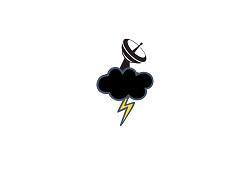
\includegraphics[width=9cm]{images/mobicharged.png} 
}
\author{Team Super Charged (No.33)
		\\ Nashit Mohammad - mohamn31
		\\ Eric Nguyen - nguyee13
		\\ Samuel De Haan - dehaas1
		\\ Eamon Earl - earle2
		\\ Mustafa Choueib - choueibm
}
    

\date{November 2nd, 2022}


\maketitle

\pagenumbering{roman}
\tableofcontents
\listoffigures
\listoftables

\vspace{20pt}


\newpage

\pagenumbering{arabic}

\section{Revision History}
\begin{center}
\begin{table}[H]
\caption{\bf Revision History}
    \begin{tabular}{p{2cm}p{3cm}p{2cm}p{6cm}}
    \hline
    \bf Author & \bf Date & \bf Version & \bf Description\\
    \hline
    All & March 8th, 2023 & Rev 0 & Created first draft of document\\
    \hline
    Mustafa Choueib & March 9th, 2023 & Rev 1 & Fixed formatting issues, revised tex document, and made grammatical corrections\\
    \hline
    \end{tabular}
\end{table}
\end{center}


\section{Definitions}
\begin{table}[H]
\caption{\bf Naming Conventions and Terminology}
\begin{tabular}{ |p{6cm}|p{8cm}|  } 
 \hline
\bf Word & \bf Definition/Context\\
 \hline
 Functional Requirement & Requirements that describe what the product is supposed to do\\
 \hline
Non-functional Requirement & Requirements that describe qualities that product will have\\
\hline
Data Smoothing & The process of using old data as well as "future" data in order to predict designs.\\
\hline
ML & "Machine Learning" algorithm.\\
\hline
SRS & Software Requirements Specification\\
\hline
Cryptography & The practice and study of techniques for secure communication\\
\hline
Asymmetric Key Cryptography & An encryption and decryption system that includes a public and private key pair\\
\hline
Functional Testing & Type of software testing that validates the software system against the functional requirements/specifications\\
\hline
Structural Testing & Type of software testing that uses the internal design of the software\\
\hline
Dynamic Testing & Test cases that are executed at run-time\\
\hline
Static Testing & Testing that does not require program execution\\
\hline
Manual Testing & Tests written and executed manually by team members\\
\hline
Automated Testing & Testing that makes use of software tools that execute tests automatically\\
\hline
System Testing & Testing that tests the system as a completed program and is based on the requirements\\
\hline
PROCESS-BENCHMARK & The average time required for completion of the current process (6 hours)\\
\hline
MAX-CHARGE-TIME & The maximum allowed time required to remotely charge a target device (4 hours)\\
\hline
\end{tabular}
\end{table}

\section{Objective}
The objective in this document is to establish a validate \& verify of certain aspects of the system that correlate with the successful completion of satisfying requirements as well as ensuring the system is built as per intentions. The key objective with this document is to build confidence in the outputs produced by the Mobicharged system as well as establish confirmation of ease of navigation for our users when using the system. A selected key objective that should not be ignored is the aim to not only output application variables that will work successfully for the application, but to specifically output the most optimized solution.

\section{Functional Requirements Evaluation}
To ensure the system satisfies what it was intended to do, it was verified in relation to the SRS document; in particular section 9, \emph{Functional Architecture}. In conjunction, the plan outlined in the V\&V Plan document section 4, \emph{System Test Description}, was used to guide testing. Evaluation of the functional requirements can be found in Section 5. Tests were run to determine successful completion of requirements. 

\begin{center}
    \begin{itemize}
        \item \textbf{SR1: ML Model must optimize inputs faster than the existing process}
        \item \textbf{SR2: ML Model must be able to develop "new" simulations based on previous optimal models}
        \item \textbf{SR3: ML Model must be able to encrypt optimized data before exporting}
        \item \textbf{SR4: The software system must determine and output optimized and correct solution}
        \item \textbf{SR5: ML Model must be able to process incoming simulation data from multiple source devices}
        \item \textbf{SR6: ML Model must be able to interpret data exported directly from MATLAB simulations}
        \item \textbf{HR1: The system must be able to use Phased-Wave interference to produce a visual output}
        \item \textbf{HR2: The system must be able to provide data to an external system}
    \end{itemize}
\end{center}

\section{Non-Functional Requirements Evaluation}
In the same vein as the functional requirement evaluation, it was verified in relation to the SRS document; in particular to section 9, \emph{Functional Architecture}. In conjunction, the plan outlined in the V\&V Plan document section 4, \emph{System Test Description}, was used to guide testing.
\par
In certain cases where the non-functional requirements pertains to a non-quantifiable attribute, testing was not applicable (i.e, APR1). In these cases, group, supervisor, and peer feedback were taken in a casual constructive form.

\begin{center}
    \begin{itemize}
        \item \textbf{APR1: The system will consist of a simple user interface}
        \item \textbf{ACR1: Authorized users will have access to the system}
        \item \textbf{IR1: The system must be able to store its current state locally in the event of a failure}
        \item \textbf{IR2: The individual components of the physical system must be inspected and tested}
        \item \textbf{EUR1: The system shall be easy to use}
        \item \textbf{EUR2: The system shall be easy to install}
        \item \textbf{LR1: The system shall be understandable within an hour of use}
        \item \textbf{SLR1: The system must compute optimal configuration within 6 hours}
        \item \textbf{PAR1: The system must have a relative accuracy of 5\% compared to current MATLAB simulation}
        \item \textbf{RAR1: The system must be available at all times}
        \item \textbf{RFTR1: The system must be able to discard any corrupted data without adding it to the database}
        \item \textbf{PER1: The hardware system must be able to withstand harsh weather}
        \item \textbf{ADAR1: The system must be functional on all operating systems}
        \item \textbf{PVR1: The system must encrypt all exported data}
    \end{itemize}
\end{center}

\section{Background}
\subsection{Software System}
The purpose of the software system, MobiCharged, is a machine learning algorithm that will be used by Mobilite-Power, engineering consultant groups, general contractors, and building maintenance teams to optimize the design process required to effectively and efficiently produce the most viable remote charging system. In doing so, this will negate the current process of manually conducting simulations (that requires lengthy computerized numerical calculations), ultimately minimizing cost, manual labour, and the time necessary to produce the required results.
\par
This system will provide users with the optimal configuration of a remote charging device based on the desired output, encrypt data protecting users when producing design results, and use data smoothing to ensure the accuracy of the system in a time efficient manner.

\subsection{Hardware System}
The purpose of the hardware system is to root our algorithms optimization in the real world environment. The production of a physical model will assist in determination of the absolute boundaries that can be fed into the machine learning algorithm. Variable parameter ranges will be derived from the physical model to determine the magnitude to which the boundaries can be pushed within the simulation. The physical system provides a secondary purpose in the form of data collection and verification. In order to increase the breadth of data that we can feed into the algorithm, we must determine the degree of computational error within the simulation results. A physical model will aid in determining this range and lead to further optimization through the machine learning algorithm.

\section{Test Cases}
\subsection{Hardware Test Cases}

\begin{table}[H]
\caption{\bf Hardware Test Cases}
\begin{tabular}{ |p{1cm}|p{2.2cm}|p{2.4cm}|p{2cm}|p{1.7cm}|p{1.7cm}|p{1.7cm}|p{1.3cm}|  } 
 \hline
\bf Test Number & \bf Description & \bf Requirement Reference & \bf Modules Referenced & \bf Inputs & \bf Expected Outputs & \bf Actual Outputs & \bf Results\\
 \hline
 1. & Hardware visual effectiveness test & HR1 & HW Power Supply, HW Microcontroller, HW Transducer Circuitry & Styrofoam ball & Levitation of object & Levitation of object & Pass\\
 \hline
 2. & Hardware visual effectiveness test & HR1 & HW Power Supply, HW Microcontroller, HW Transducer Circuitry & Plastic ball & Levitation of object & No levitation of object  & Fail\\
 \hline
\end{tabular}
\end{table}

\subsection{Software Test Cases}
\begin{center}
\begin{table}[H]
\centering
\begin{tabular}{ |p{5cm}|p{10cm}|  } 
 \hline
\bf Component & \bf Test Plan Test Factors\\
\hline
 Server-Side Application & The main reason for testing the server-side application is to ensure that the server is launching correctly, allowing/accepting access given the connection is authorized, receiving input/output pairs from the client, communicating and transferring data to the database, generating new random input to send back to the client autonomously, and storing data to a local database that is kept until a data transfer is initiated. Aspects of the application that exhibit the same or similar functionality were grouped and tested. For example, initialization of the server was tested as a group. In addition to this, groups were tested sequentially in the order they would typically execute.\\
\hline
Client-Side Application & The main reason for testing the client-side application is to ensure that a client is able to calculate simulation results, connect to the server, and transmit and receive data to and from the server. Thus, the majority of testing is done to ensure correctness and reliability of the client-side application to ensure that it is operating as intended. The way the client-side application was tested is similar to the testing plan of the server-sided application. Different functions within this application were grouped and tested sequentially based on the order they would normally execute. The testing consisted mainly of testing the communication between the client and server, and ensuring the expected data being transferred and received was correct.\\
\hline
Server Initializer Application & The main reason for testing the server initializer is to ensure that the server will never start up with broken or incorrect configurations. This application is basically testing input types and ensuring that all the values passed in are parsed correctly and are the expected types.\\
\hline
\end{tabular}
\caption{\bf Software Server-Client Components}
\label{tab:my_label}
\end{table}
\end{center}


\fancyhf{}
\fancyhead[C]{\thepage}
\renewcommand{\headrulewidth}{0pt}
\pagestyle{plain}

\subsubsection{Server-Side Initializer Application}
\begin{center}
    \begin{table}[H]
        \centering
        \begin{tabular}{|p{1cm}|p{2.2cm}|p{2.5cm}|p{1.7cm}|p{2.6cm}|p{2.6cm}|p{1.5cm}|}
        \hline
        \bf Test Number & \bf Description & \bf Requirement Reference & \bf Inputs & \bf Expected Outputs & \bf Actual Outputs & \bf Results \\
        \hline
        1. & Testing initial server configuration (\# of unique inputs, \# of unique outputs, range for input 1,2,3, and 4) & N/A & 4,3,\newline [1,2],[3,4], \newline [5,6],[7,8] & inputSize == 4 \&\& outputSize == 3 \&\& inputList == [[1,2],[3,4],[5,6],\newline [7,8]] & inputSize == 4 \&\& outputSize == 3 \&\& intputList == [[1,2],[3,4],[5,6],\newline [7,8]] & Pass\\
        \hline
        2. & Testing that initial server configuration only accepts integer values & N/A & a,b,c,d,e,f,\newline g,h,i,j & "Please enter an integer value" prompt & "Please enter an integer value" prompt & Pass\\
        \hline
        \end{tabular}
        \caption{Server-Side Initializer Test Cases}
        \label{tab:my_label1}
    \end{table}
\end{center}
\fancyhf{}
\fancyhead[C]{\thepage}
\renewcommand{\headrulewidth}{0pt}
\pagestyle{plain}



\subsubsection{Server-Side Application}
\newpage
\begin{center}
    \begin{table}[H]
        \centering
        \begin{tabular}{|p{1cm}|p{2.2cm}|p{2.5cm}|p{2.6cm}|p{2.5cm}|p{2.5cm}|p{1.3cm}|}
        \hline
        \bf Test Number & \bf Description & \bf Requirement Reference & \bf Inputs & \bf Expected Outputs & \bf Actual Outputs & \bf Results \\
        \hline
        1. & Testing that the server checks local database and acknowledges it is empty & IR1 & Local database is empty & "Clean Local Database, Current Queue is empty!" prompt & "Clean Local database, Current Queue is empty!" prompt & Pass\\
        \hline
        2. & Testing that the server retrieves the data inside the local database when it is not empty & IR1 & Local Database = \{\{'ID': '884a5913-47a1-4610-bda4-5db03aa8f425', 'Input': [1.69987008\newline94027414,3.6\newline88886129396\newline8028,1.09399\newline82029550088\newline,3.325165892\newline7677354],\newline'Output': 13\},\{'ID':'7c\newline f59c41-acb3-4e03-9ade-6f7235c7ca97\newline','Input':[1.47\newline963341984527\newline2,3.10597539\newline27838574,1.07\newline95084653703\newline89,3.4097349\newline62180615],\newline'Output':13\}\} & output\_q == [\{\{'ID': '884a5913-47a1-4610-bda4-5db03aa8f425', 'Input': [1.69987008\newline94027414,3.6\newline88886129396\newline8028,1.09399\newline82029550088\newline,3.325165892\newline7677354],\newline'Output': 13\},\{'ID':'7c\newline f59c41-acb3-4e03-9ade-6f7235c7ca97\newline','Input':[1.47\newline963341984527\newline2,3.10597539\newline27838574,1.07\newline95084653703\newline89,3.4097349\newline62180615],\newline'Output':13\}\}] & output\_q == [\{\{'ID': '884a5913-47a1-4610-bda4-5db03aa8f425', 'Input': [1.69987008\newline94027414,3.6\newline88886129396\newline8028,1.09399\newline82029550088\newline,3.325165892\newline7677354],\newline'Output': 13\},\{'ID':'7c\newline f59c41-acb3-4e03-9ade-6f7235c7ca97\newline','Input':[1.47\newline963341984527\newline2,3.10597539\newline27838574,1.07\newline95084653703\newline89,3.4097349\newline62180615],\newline'Output':13\}\}] & Pass\\
        \hline
        \end{tabular}
        \caption{Server-Side Test Cases (1-2)}
        \label{tab:my_label2}
    \end{table}
\end{center}

\fancyhf{}
\fancyhead[C]{\thepage}
\renewcommand{\headrulewidth}{0pt}
\pagestyle{plain}


\begin{center}
    \begin{table}[H]
        \centering
        \begin{tabular}{|p{1cm}|p{2.2cm}|p{2.5cm}|p{2.7cm}|p{2.4cm}|p{2.4cm}|p{1.3cm}|}
        \hline
        \bf Test Number & \bf Description & \bf Requirement Reference & \bf Inputs & \bf Expected Outputs & \bf Actual Outputs & \bf Results \\
        \hline
        3. & Testing that the server is appending each new input/output pair to the local database & IR1 & pair =\{'ID':'7vq92b\newline61-bdc8-1y15-9jqh-4f4367b3ba97',\newline'Input':[1.46318\newline79642130127,3.5\newline67941357964125\newline4,1.5786135784\newline296312,3.96347\newline81254631236],\newline'Output': 10\} & Local Database = \{\{'ID':'7vq92b\newline61-bdc8-1y15-9jqh-4f4367b3ba97'\newline,'Input':[1.463\newline187964213012\newline7,3.567941357\newline9641254,1.578\newline613578429631\newline2,3.963478125\newline4631236],\newline'Output': 10\}\} & Local Database = \{\{'ID':'7vq92b\newline61-bdc8-1y15-9jqh-4f4367b3ba97'\newline,'Input':[1.463\newline187964213012\newline7,3.567941357\newline9641254,1.578\newline613578429631\newline2,3.963478125\newline4631236],\newline'Output': 10\}\} & Pass \\
        \hline
        4. & Testing that the server can handle a client connection & ACR1 & Client requests connection & connected\_clie\newline nts[0][0] = ('99.235.234\newline.43') & connected\_clie\newline nts[0][0] = ('99.235.234\newline.43') & Pass\\
        \hline
        5. & Testing that the server can handle multiple client connections & ACR1 & Multiple clients request connection & connected\_clie\newline nts[0][0] = [('99.235.234\newline.43'), ('99.235.234\newline.43')] & connected\_clie\newline nts[0][0] = [('99.235.234\newline.43'), ('99.235.234\newline.43')] & Pass\\
        \hline
        \end{tabular}
        \caption{Server-Side Test Cases (3-5)}
        \label{tab:my_label3}
    \end{table}
\end{center}

\fancyhf{}
\fancyhead[C]{\thepage}
\renewcommand{\headrulewidth}{0pt}
\pagestyle{plain}

\begin{center}
    \begin{table}[H]
        \centering
        \begin{tabular}{|p{1cm}|p{2.2cm}|p{2.5cm}|p{2.7cm}|p{2.4cm}|p{2.4cm}|p{1.3cm}|}
        \hline
        \bf Test Number & \bf Description & \bf Requirement Reference & \bf Inputs & \bf Expected Outputs & \bf Actual Outputs & \bf Results \\
        \hline
        6. & Testing that the server can handle multiple client connections & ACR1 & 4  clients request connection & len(connected\newline\_clients) == 4 & len(connected\newline\_clients) == 4 & Pass\\
        \hline
        7. & Testing that the server rejects incorrect authorization from the client & ACR1 & Client sends incorrect authorization message & authSucecss == False \&\& "Incorrect Authorization key, disconnecting!" prompt & authSucecss == False \&\& "Incorrect Authorization key, disconnecting!" & Pass\\
        \hline
        8. & Testing that the server accepts correct authorization from the client & ACR1 & Client sends correct authorization message & authSuccess == True \&\& connected\newline \_clients[0][0] == ('99.235.234.\newline43') \&\& "Correct Authorization key, Accepting Connection!" prompt & authSuccess == True \&\& connected\newline\_clients[0][0] == ('99.235.234.\newline43') \&\& "Correct Authorization key, Accepting Connection!" prompt & Pass\\
        \hline
        9. & Testing that the server can receive input from the client & N/A & Client sends optimal output to server == 10.0 & received\_data.\newline pickleloads(re\newline ceived\_data) == 10 & received\_data.\newline pickleloads(re\newline ceived\_data) == 10 & Pass\\
        \hline
        \end{tabular}
        \caption{Server-Side Test Cases (6-9)}
        \label{tab:my_label4}
    \end{table}
\end{center}

\fancyhf{}
\fancyhead[C]{\thepage}
\renewcommand{\headrulewidth}{0pt}
\pagestyle{plain}

\begin{center}
    \begin{table}[H]
        \centering
        \begin{tabular}{|p{1cm}|p{2.2cm}|p{2.5cm}|p{2.7cm}|p{2.4cm}|p{2.4cm}|p{1.3cm}|}
        \hline
        \bf Test Number & \bf Description & \bf Requirement Reference & \bf Inputs & \bf Expected Outputs & \bf Actual Outputs & \bf Results \\
        \hline
        10. & Testing that the server generates new input within the range specified on launch & SR2 & Server receives optimal output \&\& output\_q.isFull() == False & (1 \leq newResponse\newline[0] \leq 2 \&\& 3 \leq newResponse\newline[1] \leq 4 \&\& 5 \leq newResponse\newline[2] \leq 6 \&\& 7 \leq newResponse\newline[3] \leq 8) == True & (1 \leq newResponse\newline[0] \leq 2 \&\& 3 \leq newResponse\newline[1] \leq 4 \&\& 5 \leq newResponse\newline[2] \leq 6 \&\& 7 \leq newResponse\newline[3] \leq 8) == True & Pass\\
        \hline
        11. & Testing that the server calls for a data transfer once the output\_q is full & SR3 & output\_q.isFull() == True \&\& received\_data & Local Database.\newline isEmpty() == True & Local Database.\newline isEmpty() == True & Pass\\
        \hline
        12. & Testing that the server does not lose data if interrupted during data transfer & RFTR1 & output\_q = \{1,2,3,4,5,6,7,\newline 8,9,10\} \&\& finished transferring \{1,2,3,4\} then interrupted during the 5th value & continue transfer from output\_q == \{5,6,7,8,9,10\} & continue transfer from output\_q == \{1,2,3,4,5,6,7,\newline8,9,10\} & Fail\\
        \hline
        \end{tabular}
        \caption{Server-Side Test Cases (10-12)}
        \label{tab:my_label5}
    \end{table}
\end{center}
\fancyhf{}
\fancyhead[C]{\thepage}
\renewcommand{\headrulewidth}{0pt}
\pagestyle{plain}


\begin{center}
    \begin{table}[H]
        \centering
        \begin{tabular}{|p{1cm}|p{2.2cm}|p{2.5cm}|p{2.7cm}|p{2.4cm}|p{2.4cm}|p{1.3cm}|}
        \hline
        \bf Test Number & \bf Description & \bf Requirement Reference & \bf Inputs & \bf Expected Outputs & \bf Actual Outputs & \bf Results \\
        \hline
        13. & Testing if the server is functional on all operating systems & ADAR1 & Running the server-side application on multiple operating systems & "Mobicharged is now running" prompt on all devices & "Mobicharged is now running" prompt on all devices & Pass\\
        \hline
        \end{tabular}
        \caption{Server-Side Test Cases (13)}
        \label{tab:my_label6}
    \end{table}
\end{center}

\subsubsection{Client Side Application}

\begin{center}
    \begin{table}[H]
        \centering
        \begin{tabular}{|p{1cm}|p{2.2cm}|p{2.5cm}|p{2.7cm}|p{2.4cm}|p{2.4cm}|p{1.3cm}|}
        \hline
        \bf Test Number & \bf Description & \bf Requirement Reference & \bf Inputs & \bf Expected Outputs & \bf Actual Outputs & \bf Results \\
        \hline
        1. & Testing that the client-side application attempts to connect to the server & N/A & Python client\newline\_controller.py & "Please enter the authorization key: " prompt & "Please enter the authorization key: " prompt & Pass\\
        \hline
        2. & Testing that the client-side application is refused connection if failed authorization & ACR1 & authorizationKey  = "incorrectpassword" & "Authorization Failed. Disconnecting." prompt & "Authorization Failed. Disconnecting" prompt & Pass\\
        \hline
        3. & Testing that the client-side application is accepted connection on successful authorization & ACR1 & AuthorizationKey = "mobicharged" & "Authorization Successful, Connecting to server" prompt & "Authorization Successful, Connecting to server" prompt & Pass\\
        \hline
        \end{tabular}
        \caption{Client-Side Test Cases (1-3)}
        \label{tab:my_label7}
    \end{table}
\end{center}
\fancyhf{}
\fancyhead[C]{\thepage}
\renewcommand{\headrulewidth}{0pt}
\pagestyle{plain}

\begin{center}
    \begin{table}[H]
        \centering
        \begin{tabular}{|p{1cm}|p{2.2cm}|p{2.5cm}|p{2.7cm}|p{2.4cm}|p{2.4cm}|p{1.3cm}|}
        \hline
        \bf Test Number & \bf Description & \bf Requirement Reference & \bf Inputs & \bf Expected Outputs & \bf Actual Outputs & \bf Results \\
        \hline
        4. & Testing that the client-side application prompts user to input an initial value to start autonomous chain & SR2 & Connection is successfully established & "Input parameter for the optimization problem:" prompt & "Input parameter for the optimization problem:" prompt & Pass\\
        \hline
        5. & Testing that the client-side application must take a float value for the initial input & SR2 & initial\_input = "StringInsteadOfFloat" & "Input must be numeric 0-9" prompt & "Input must be numeric 0-9" prompt & Pass\\
        \hline
        6. & Testing that the client-side application takes the input in "inputParams" and starts a MATLAB simulation & N/A & initial\_input = [30.0,40.0,\newline50.0,60.0] & MATLAB simulation is ran given the initial\_input as parameters & MATLAB simulation is ran given the initial\_input as parameters & Pass\\
        \hline
        \end{tabular}
        \caption{Client-Side Test Cases (4-6)}
        \label{tab:my_label8}
    \end{table}
\end{center}

\begin{center}
    \begin{table}[H]
        \centering
        \begin{tabular}{|p{1cm}|p{2.2cm}|p{2.5cm}|p{2.7cm}|p{2.4cm}|p{2.4cm}|p{1.3cm}|}
        \hline
        \bf Test Number & \bf Description & \bf Requirement Reference & \bf Inputs & \bf Expected Outputs & \bf Actual Outputs & \bf Results \\
        \hline
        7. & Testing that the client-side application receives and optimal value from the MATLAB simulation & N/A & initial\_input = [30.0,40.0,\newline50.0,60.0] & MATLAB simulation is ran with initial\_input as parameters \&\& optimal\_output = 10.0 (hard coded response from MATLAB for testing) & MATLAB simulation is ran with initial\_input as parameters \&\& optimal\_output = 10.0 (hard coded response from MATLAB for testing) & Pass\\
        \hline
        8. & Testing that the client-side application provides a uniqueID to eery optimal output produced by MATLAB & N/A & Received optimal\_output = 10.0 from MATLAB & Data["ID"] != Null & Data["ID"] != Null & Pass\\
        \hline
        9. & Testing that the client-side application sends the input/output pair to the server & N/A & data\_string = pickle.\newline dumps(data) \&\& soc.\newline send(data\_\newline string) & Manual Check: received\_data 1= Null (on server side) & Manual Check: received\_data != Null (on server side) & Pass\\
        \hline
        \end{tabular}
        \caption{Client-Side Test Cases (7-9)}
        \label{tab:my_label9}
    \end{table}
\end{center}

\begin{center}
    \begin{table}[H]
        \centering
        \begin{tabular}{|p{1cm}|p{2.2cm}|p{2.5cm}|p{2.7cm}|p{2.4cm}|p{2.4cm}|p{1.3cm}|}
        \hline
        \bf Test Number & \bf Description & \bf Requirement Reference & \bf Inputs & \bf Expected Outputs & \bf Actual Outputs & \bf Results \\
        \hline
        10. & Testing that the client-side application receives new input from the server & SR2 & soc.\newline send(data\_string) & data\_received != Null & data\_received != Null & Pass\\
        \hline
        11. & Testing that the client-side application computes optimal configuration within 6 hours & SLR1 & y = eng.unknown\_\newline poly\_type\newline (inputParams, nargout = 1) \&\& start_stopwatch & (Elapsed\_time \leq 21600 \newline (seconds)) == True & (Elapsed\_time \leq 21600 \newline (seconds)) == True & Pass\\
        \hline
        \end{tabular}
        \caption{Client-Side Test Cases (10-11)}
        \label{tab:my_label10}
    \end{table}
\end{center}

\subsubsection{Database Module Test Cases}
\begin{center}
\begin{table}[H]
\centering
\begin{tabular}{ |p{5cm}|p{10cm}|  } 
 \hline
\bf Component & \bf Test Plan Test Factors\\
\hline
 Database Module & The database module requires testing to ensure that the functionality of the database module and that both the Server-Client and Machine Learning Blackboard module are able to communicate with it. Examples of the aspects being tested are the backup/recovery abilities of the database in the scenario of a major failure, and correct data formatting/indexing of all read/write functions.\\
 \hline
\end{tabular}
\caption{\bf Database Components}
\label{tab:my_label11}
\end{table}
\end{center}

\begin{center}
    \begin{table}[H]
        \centering
        \begin{tabular}{|p{1cm}|p{2.2cm}|p{2.5cm}|p{2.7cm}|p{2.4cm}|p{2.4cm}|p{1.3cm}|}
        \hline
        \bf Test Number & \bf Description & \bf Requirement Reference & \bf Inputs & \bf Expected Outputs & \bf Actual Outputs & \bf Results \\
        \hline
        1. & Test server connection. Determine if the server module is able to write to the database & RAR1 & [ID:”006dd8fc-44f3-4e9a-9b15-e12557df1a48”,\newline Input:{0:1,1:2,2:3,\newline3:4},\newline Output:1.21922\newline2] & A new document is added to the "MATLAB\_Simula\newline tions" collection & A new document is added to the "MATLAB\_Simula\newline tions" collection & Pass\\
        \hline
        2. & Test client connection. Determine if the client module is able to read from the database & RAR1 & Call batched\_read() & Returns a dictionary containing all stored data in database & Returns a dictionary containing all stored data in database (tested with 1 entry and with 1000 entries) & Pass\\
        \hline
        3. & Test security protocol of Firestore. Ensure that non-authorized users are unable to read/write to database & ACR1 & Call batched\_read() without Firestore authentication & "Unauthorized request" prompt & "Unauthorized request" prompt & Pass\\
        \hline
        \end{tabular}
        \caption{Database Test Cases (1-3)}
        \label{tab:my_label12}
    \end{table}
\end{center}

\begin{center}
    \begin{table}[H]
        \centering
        \begin{tabular}{|p{1cm}|p{2.2cm}|p{2.5cm}|p{2.7cm}|p{2.4cm}|p{2.4cm}|p{1.3cm}|}
        \hline
        \bf Test Number & \bf Description & \bf Requirement Reference & \bf Inputs & \bf Expected Outputs & \bf Actual Outputs & \bf Results \\
        \hline
        4. & Test data structure consistency during read/write functions. Ensure that the data being written to the database has the same data structure as data being read & N/A & N/A & [ID:”006dd8fc-44f3-4e9a-9b15-e12557df1a48”, Input:{0:1,1:2,2:3\newline,3:4},\newline Output:1.219\newline222] is written and read & [ID:”006dd8fc-44f3-4e9a-9b15-e12557df1a48”, Input:{0:1,1:2,2:3\newline,3:4},\newline Output:1.219\newline222] is written and read & Pass\\
        \hline
        5. & Test backup and recovery capabilities. In the case of a corrupted database, make sure that a local copy or previous version can be reestablished & RAR1 & Call recover\_last\_\newline db\_version() & Wipes corrupted dataset and re-writes most recently stored database & Wipes corrupted dataset and re-writes most recently stored database & Pass\\
        \hline
        \end{tabular}
        \caption{Database Test Cases (4-5)}
        \label{tab:my_label13}
    \end{table}
\end{center}

\begin{center}
    \begin{table}[H]
        \centering
        \begin{tabular}{|p{1cm}|p{2.2cm}|p{2.5cm}|p{2.7cm}|p{2.4cm}|p{2.4cm}|p{1.3cm}|}
        \hline
        \bf Test Number & \bf Description & \bf Requirement Reference & \bf Inputs & \bf Expected Outputs & \bf Actual Outputs & \bf Results \\
        \hline
        6. & Test database size funtionality. Ensure that the database is still functioning after storing a large amount of data & RAR1 \newline PER1 & \begin{enumerate}
            \item Call write\_lar\newline ge\_\newline dataset()
            \item Call batched\_\newline read()
        \end{enumerate} & Even with 1000 entries, the database read and write functions should still work & Both read and write functionalities continue to work. Output is not written because it is too large & Pass\\
        \hline
        7. & Test incorrect data structure handling. The database should reject incorrectly formatted data & RFTR1 & Call write\_data() with [ID:"12"] & "Incorrect data structure inputted. Server should input [ID:"", Input:{}, Output: \_\_]" & "Incorrect data structure inputted. Server should input [ID:"", Input:{}, Output: \_\_]" & Pass\\
        \hline
        8. & Reading data from an empty database & N/A & Call batched\_read() & "Database is empty" prompt, and returns an empty dictionary & "Database is empty" prompt, and returns an empty dictionary & Pass\\
        \hline
        \end{tabular}
        \caption{Database Test Cases (6-8)}
        \label{tab:my_label14}
    \end{table}
\end{center}

\subsubsection{Machine Learning Blackboard Test Cases}
\begin{center}
\begin{table}[H]
\centering
\begin{tabular}{ |p{5cm}|p{10cm}|  } 
 \hline
\bf Component & \bf Test Plan Test Factors\\
\hline
 Machine Learning Blackboard & The critical behaviour that we wish to test for is the synchronicity of the threads and the interwoven processes, and that their CPU sharing is fair and allows for a reasonable user experience when combined with the UI. We also want to ensure that the main loop of the machine learner works as intended; beginning once a pre-determined threshold of data has been met in the associated database, at which point that data is funneled into the model. We then want to make sure that the user-side predictive stream is opened upon model completion, and that accuracy / progress graphs are saved in the correct locations. We also want to ensure that these graphs match the processes and final outputs of the machine learner, and that the accuracy found is representative of the accuracy displayed on these graphs. We also ultimately want to ensure that the machine learning model converges and finds a relatively accurate solution. Upon full implementation of the multi-model pruning system discussed in our demo, we will also be testing that the final model was truly the best option out of all that were attempted. \textbf{*Note:} much of this behaviour requires experiential testing, as the relative accuracies and inputs to the simulations we are attempting to mimic with our machine learning model are randomly generated, and as such can't be quantitatively verified. As such, the other behaviour, like creation of threads at the correct times, the execution of the learning process once the threshold has been met, and saving the graphs in the correct locations have also been experientially validated up to date, but these tests will be added to suite further into the development process.\\
 \hline
\end{tabular}
\caption{\bf Machine Learner Components}
\label{tab:my_label15}
\end{table}
\end{center}

\begin{center}
    \begin{table}[H]
        \centering
        \begin{tabular}{|p{1cm}|p{2.2cm}|p{2.5cm}|p{2.7cm}|p{2.4cm}|p{2.4cm}|p{1.3cm}|}
        \hline
        \bf Test Number & \bf Description & \bf Requirement Reference & \bf Inputs & \bf Expected Outputs & \bf Actual Outputs & \bf Results \\
        \hline
        1. & Upon pinging the DB and seeing a COUNT > current\_threshold, machine learning model is executed on current DB data points & N/A & Network response from DB & "Simulation started" prompt & "Simulation started" prompt & Pass\\
        \hline
        2. & Testing that the model terminates & N/A & DB input/output pairs & Matrix with weights of 'relative optimality' & Matrix with weights of 'relative optimality' & Pass on some functions, fails on others\\
        \hline
        3. & Testing whether the model generates an accuracy / epoch graph and saves it locally & N/A & DB input/output pairs & New local .jpg file showing the accuracy over epochs & New local .jpg file showing the accuracy over epochs & Pass\\
        \hline
        \end{tabular}
        \caption{Machine Learning Blackboard Test Cases (1-3)}
        \label{tab:my_label16}
    \end{table}
\end{center}

\begin{center}
    \begin{table}[H]
        \centering
        \begin{tabular}{|p{1cm}|p{2.2cm}|p{2.5cm}|p{2.7cm}|p{2.4cm}|p{2.4cm}|p{1.3cm}|}
        \hline
        \bf Test Number & \bf Description & \bf Requirement Reference & \bf Inputs & \bf Expected Outputs & \bf Actual Outputs & \bf Results \\
        \hline
        4. & Testing that the predictive stream is opened on completion of the learning process & N/A & None & "Please input your desired values on which you'd like to predict:" prompt & "Please input your desired values on which you'd like to predict:" prompt & Pass\\
        \hline
        5. & Testing that upon completion of the learning process, the module starts poling the DB again & N/A & None & Current DB count & Current DB count & Pass\\
        \hline
        6. & Testing that the predictive stream call/response from the user is not stalled by parallel computations, or consistently responds in a reasonable amount of time (\le 5s) & N/A & None & None & None & Fail - Stalls on startup without indication to user\\
        \hline
        \end{tabular}
        \caption{Machine Learning Blackboard Test Cases (4-6)}
        \label{tab:my_label17}
    \end{table}
\end{center}

\begin{center}
    \begin{table}[H]
        \centering
        \begin{tabular}{|p{1cm}|p{2.2cm}|p{2.5cm}|p{2.7cm}|p{2.4cm}|p{2.4cm}|p{1.3cm}|}
        \hline
        \bf Test Number & \bf Description & \bf Requirement Reference & \bf Inputs & \bf Expected Outputs & \bf Actual Outputs & \bf Results \\
        \hline
        7. & Testing that currently optimal model weights and current\_threshold are saved in the database after each successful pass through the learning process & N/A & [Weight Matrix, current\_threshold] & Entries entered into DB & Entries entered into DB & Pass\\
        \hline
        8. & Testing that upon new best performing model found, this model is then used in the predictive stream & N/A & None & None & None & Fail - Yet to achieve correct signalling logic\\
        \hline
        \end{tabular}
        \caption{Machine Learning Blackboard Test Cases (7-8)}
        \label{tab:my_label18}
    \end{table}
\end{center}


\begin{center}
    \begin{table}[H]
        \centering
        \begin{tabular}{|p{1cm}|p{2.2cm}|p{2.5cm}|p{2.7cm}|p{2.4cm}|p{2.4cm}|p{1.3cm}|}
        \hline
        \bf Test Number & \bf Description & \bf Requirement Reference & \bf Inputs & \bf Expected Outputs & \bf Actual Outputs & \bf Results \\
        \hline
        9. & Test that input/output numbers and boundaries set by the user through the initializer module are properly set in the predictive stream & N/A & [list of boundaries for each input] & None & None & Fail - values currently hard coded in file\\
        \hline
        10. & Testing that the currently sole model consistently produces accurate results that are correct within a 0.01 relative error rate & PAR1 & None & None & None & Pass\\
        \hline
        \end{tabular}
        \caption{Machine Learning Blackboard Test Cases (9-10)}
        \label{tab:my_label19}
    \end{table}
\end{center}


\section{Changes Due to Testing}
\subsection{Server-Client Module}
During testing, it was discovered that there is a major security flaw within the server-client connection regarding the IP addresses. A future change to improve security is to only allow clients that are connecting from an approved IP address list to connect.

\subsection{Database Module}
Previously, the Firestore database was configured to allow any user with the API key to read/write to the database. However, this was recognized to be a major security flaw and Firestore Authentication SDK was implemented to fix this. This SDK provides methods to allow users to sign in using email addresses and passwords. This user management is then used to determine which users are granted read/write permissions.

\subsection{Machine Learning Blackboard}
From the latency issues found in the predictive stream, and the cluttered messaging seen in the terminal, we found that proceeding with the development of a simple front-end system, to improve the user's ability to oversee the process of the learner, would be necessary to achieve a wholly useful project. This requirement was listed in our initial SRS (APR1), but its importance was eclipsed at the time by other services that required development. This could also help in thread management and notify updates to the predictive model, and allow the user to see progress without manually opening the saved graphical models.



\section*{References}
We will be referring to documentations provided by Mobilite-Power, however, as of now there are no references to mention.




\end{document}

